1. zhang code, generated

2. example with lists
3. complex list(add, sub) with focus on updates

\section{Scenario}
%\textcite{zhang2019scenario} 
\section{Simple Diagram with no lists}
which can be found in \code{resources/test-files/test.vue}
\begin{figure}[H]
    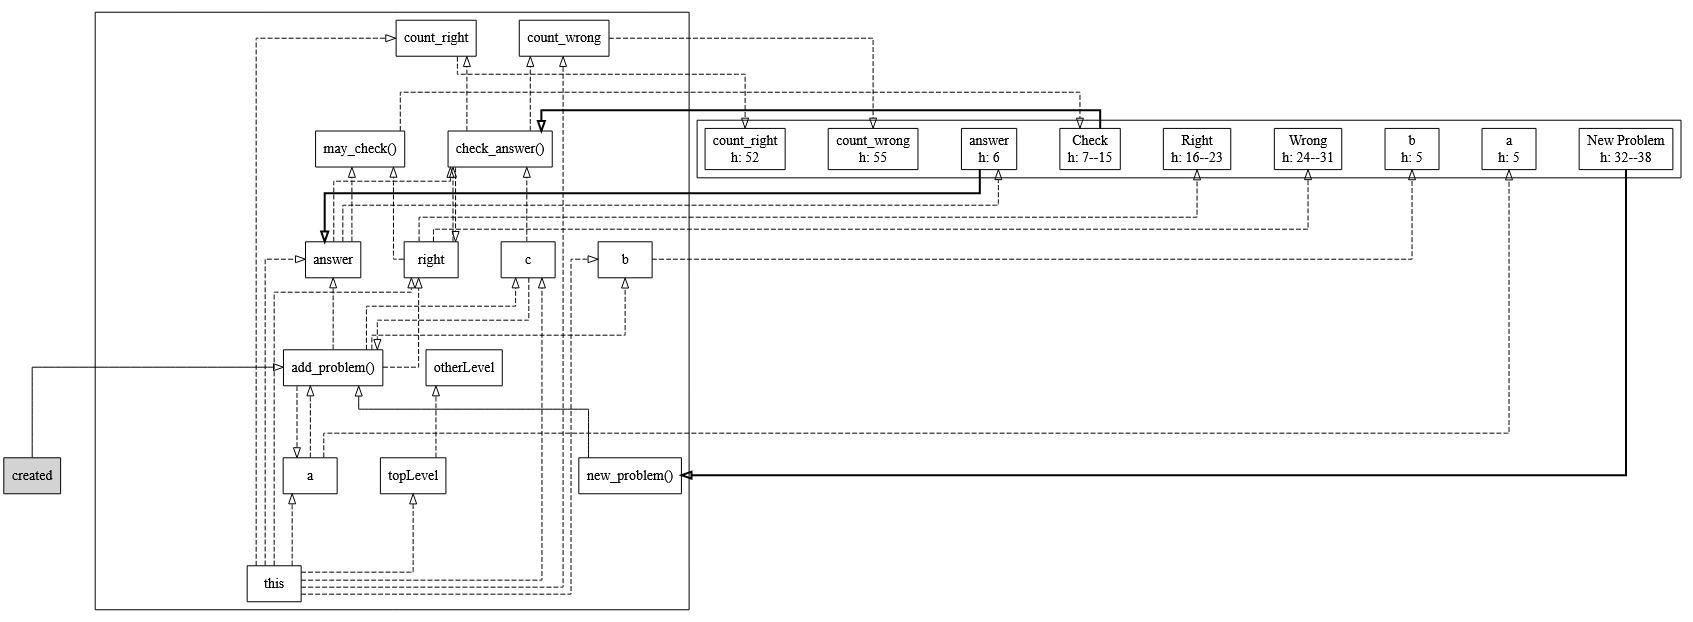
\includegraphics[width=\textwidth]{images/diagram_test_zhang.png}
     \caption{TODO }
     \label{fig:diagram_test_zhang}
\end{figure}

\section{Diagram with list}
which can be found in \code{resources/test-files/list.vue}
\begin{figure}[H]
    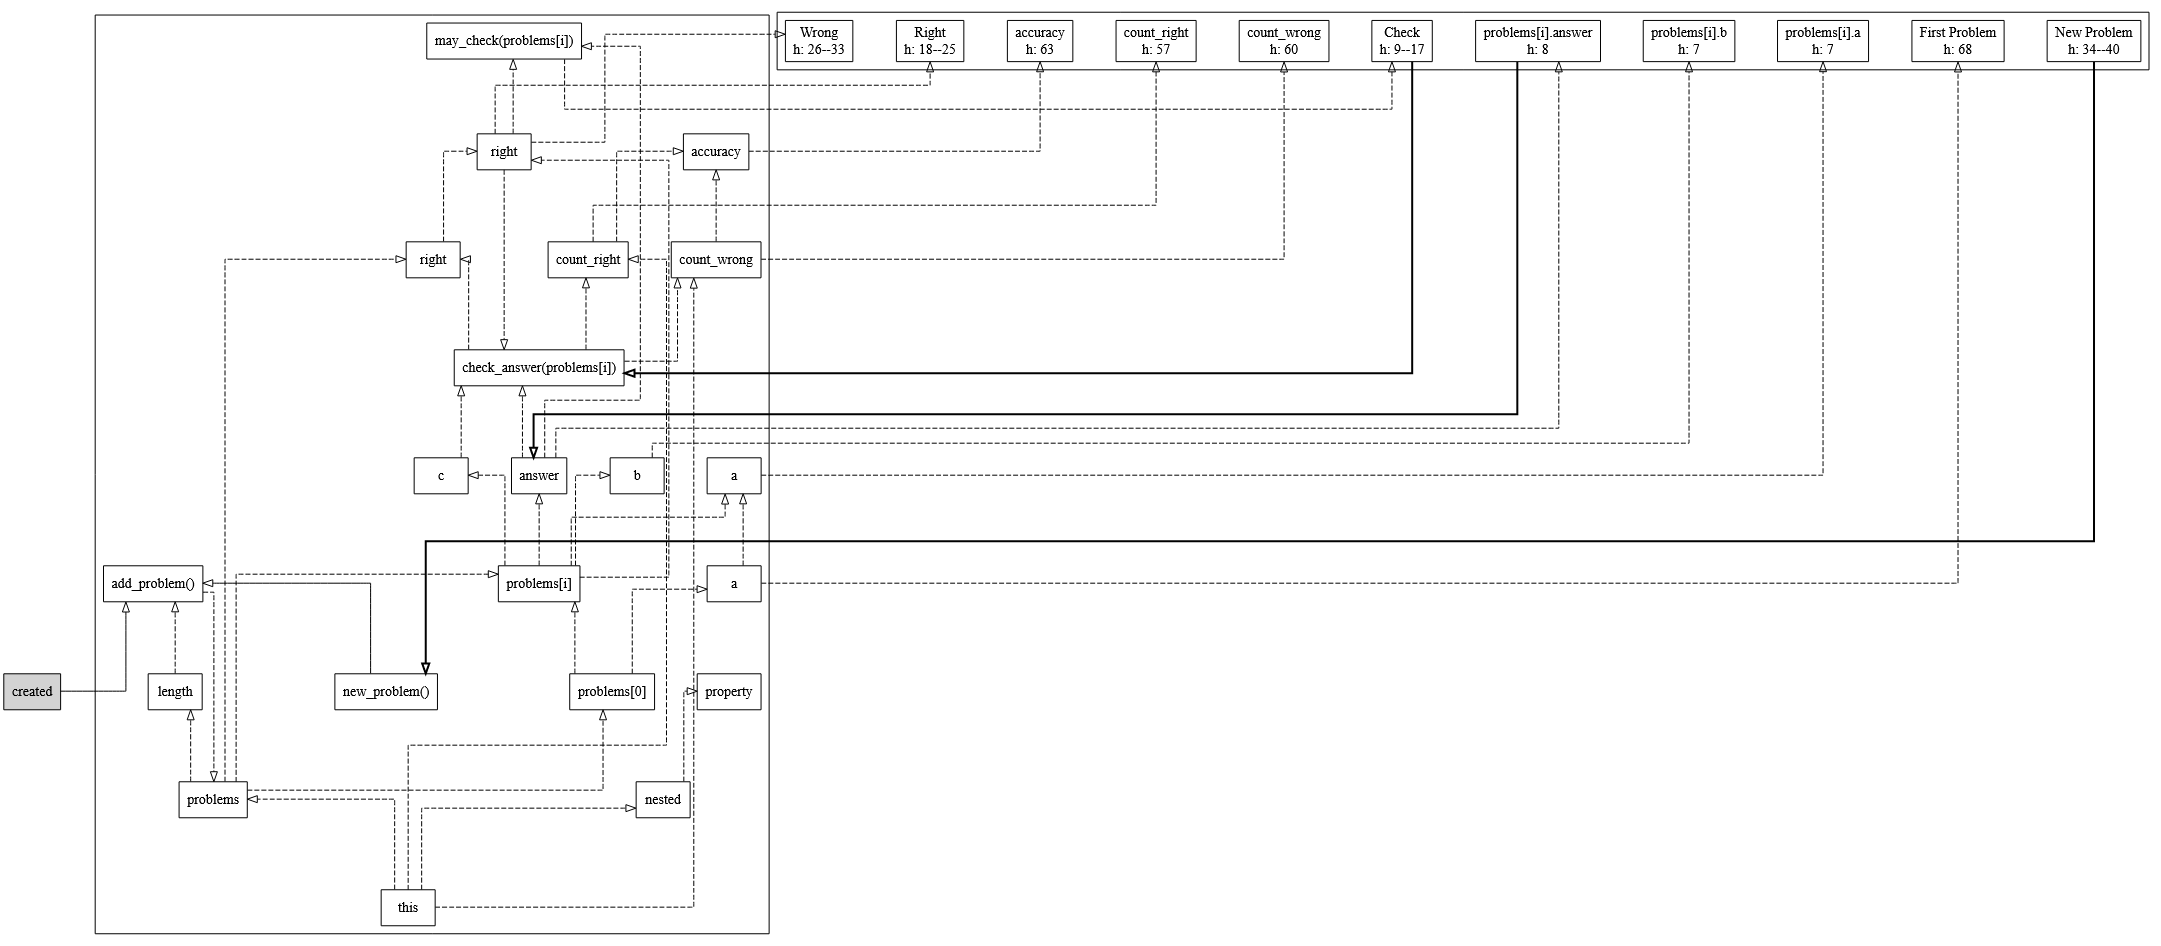
\includegraphics[width=\textwidth]{images/diagram_list.png}
     \caption{TODO}
     \label{fig:diagram_list}
\end{figure}
\begin{lstlisting}
l(answer) -> answer, Check
l(Check) -> Right, Wrong, Check, count_right, count_wrong
l(New Problem) -> a, b, answer, Check, Right, Wrong
l(created) -> a, b, answer, Check, Right, Wrong

Unique scenarios (A) of up to 4 elements:
[
[ 'created' ],
[ 'created', 'answer' ],
[ 'created', 'Check' ],
[ 'created', 'New Problem' ],
[ 'created', 'answer', 'Check' ],
[ 'created', 'New Problem', 'answer' ],
[ 'created', 'New Problem', 'Check' ],
[ 'created', 'New Problem', 'answer', 'Check' ]
]
Scenario: ['created']
When 'created'
Then 'a'
And 'b'
And 'answer'
And 'Check'
And 'Right'
And 'Wrong'

Scenario: ['created', 'answer']
Given 'created'
When 'answer'
Then 'answer'
And 'Check'

Scenario: ['created', 'Check']
Given 'created'
When 'Check'
Then 'Right'
And 'Wrong'
And 'Check'
And 'count_right'
And 'count_wrong'

Scenario: ['created', 'New Problem']
Given 'created'
When 'New Problem'
Then 'a'
And 'b'
And 'answer'
And 'Check'
And 'Right'
And 'Wrong'

Scenario: ['created', 'answer', 'Check']
Given 'created'
And 'answer'
When 'Check'
Then 'Right'
And 'Wrong'
And 'Check'
And 'count_right'
And 'count_wrong'

Scenario: ['created', 'New Problem', 'answer']
Given 'created'
And 'New Problem'
When 'answer'
Then 'answer'
And 'Check'

Scenario: ['created', 'New Problem', 'Check']
Given 'created'
And 'New Problem'
When 'Check'
Then 'Right'
And 'Wrong'
And 'Check'
And 'count_right'
And 'count_wrong'

Scenario: ['created', 'New Problem', 'answer', 'Check']
Given 'created'
And 'New Problem'
And 'answer'
When 'Check'
Then 'Right'
And 'Wrong'
And 'Check'
And 'count_right'
And 'count_wrong'


\end{lstlisting}

\begin{lstlisting}
l(problems[i].answer) -> problems[i].answer, Check
l(Check) -> Right, Wrong, Check, count_right, accuracy, count_wrong
l(New Problem) -> problems[i].a, problems[i].b, problems[i].answer, Check, Right, Wrong, First Problem
l(created) -> problems[i].a, problems[i].b, problems[i].answer, Check, Right, Wrong, First Problem

Unique scenarios (A) of up to 4 elements:
[
    [ 'created' ],
    [ 'created', 'problems[i].answer' ],
    [ 'created', 'Check' ],
    [ 'created', 'New Problem' ],
    [ 'created', 'problems[i].answer', 'Check' ],
    [ 'created', 'New Problem', 'problems[i].answer' ],
    [ 'created', 'New Problem', 'Check' ],
    [ 'created', 'New Problem', 'problems[i].answer', 'Check' ]
]
Scenario: ['created']
    When 'created'
    Then 'problems[i].a'
    And 'problems[i].b'
    And 'problems[i].answer'
    And 'Check'
    And 'Right'
    And 'Wrong'
    And 'First Problem'

Scenario: ['created', 'problems[i].answer']
    Given 'created'
    When 'problems[i].answer'
    Then 'problems[i].answer'
    And 'Check'

Scenario: ['created', 'Check']
    Given 'created'
    When 'Check'
    Then 'Right'
    And 'Wrong'
    And 'Check'
    And 'count_right'
    And 'accuracy'
    And 'count_wrong'

Scenario: ['created', 'New Problem']
    Given 'created'
    When 'New Problem'
    Then 'problems[i].a'
    And 'problems[i].b'
    And 'problems[i].answer'
    And 'Check'
    And 'Right'
    And 'Wrong'
    And 'First Problem'

Scenario: ['created', 'problems[i].answer', 'Check']
    Given 'created'
    And 'problems[i].answer'
    When 'Check'
    Then 'Right'
    And 'Wrong'
    And 'Check'
    And 'count_right'
    And 'accuracy'
    And 'count_wrong'

Scenario: ['created', 'New Problem', 'problems[i].answer']
    Given 'created'
    And 'New Problem'
    When 'problems[i].answer'
    Then 'problems[i].answer'
    And 'Check'

Scenario: ['created', 'New Problem', 'Check']
    Given 'created'
    And 'New Problem'
    When 'Check'
    Then 'Right'
    And 'Wrong'
    And 'Check'
    And 'count_right'
    And 'accuracy'
    And 'count_wrong'

Scenario: ['created', 'New Problem', 'problems[i].answer', 'Check']
    Given 'created'
    And 'New Problem'
    And 'problems[i].answer'
    When 'Check'
    Then 'Right'
    And 'Wrong'
    And 'Check'
    And 'count_right'
    And 'accuracy'
    And 'count_wrong'
\end{lstlisting}


\section{Diagram Addition and Substitution}
\begin{figure}[H]
    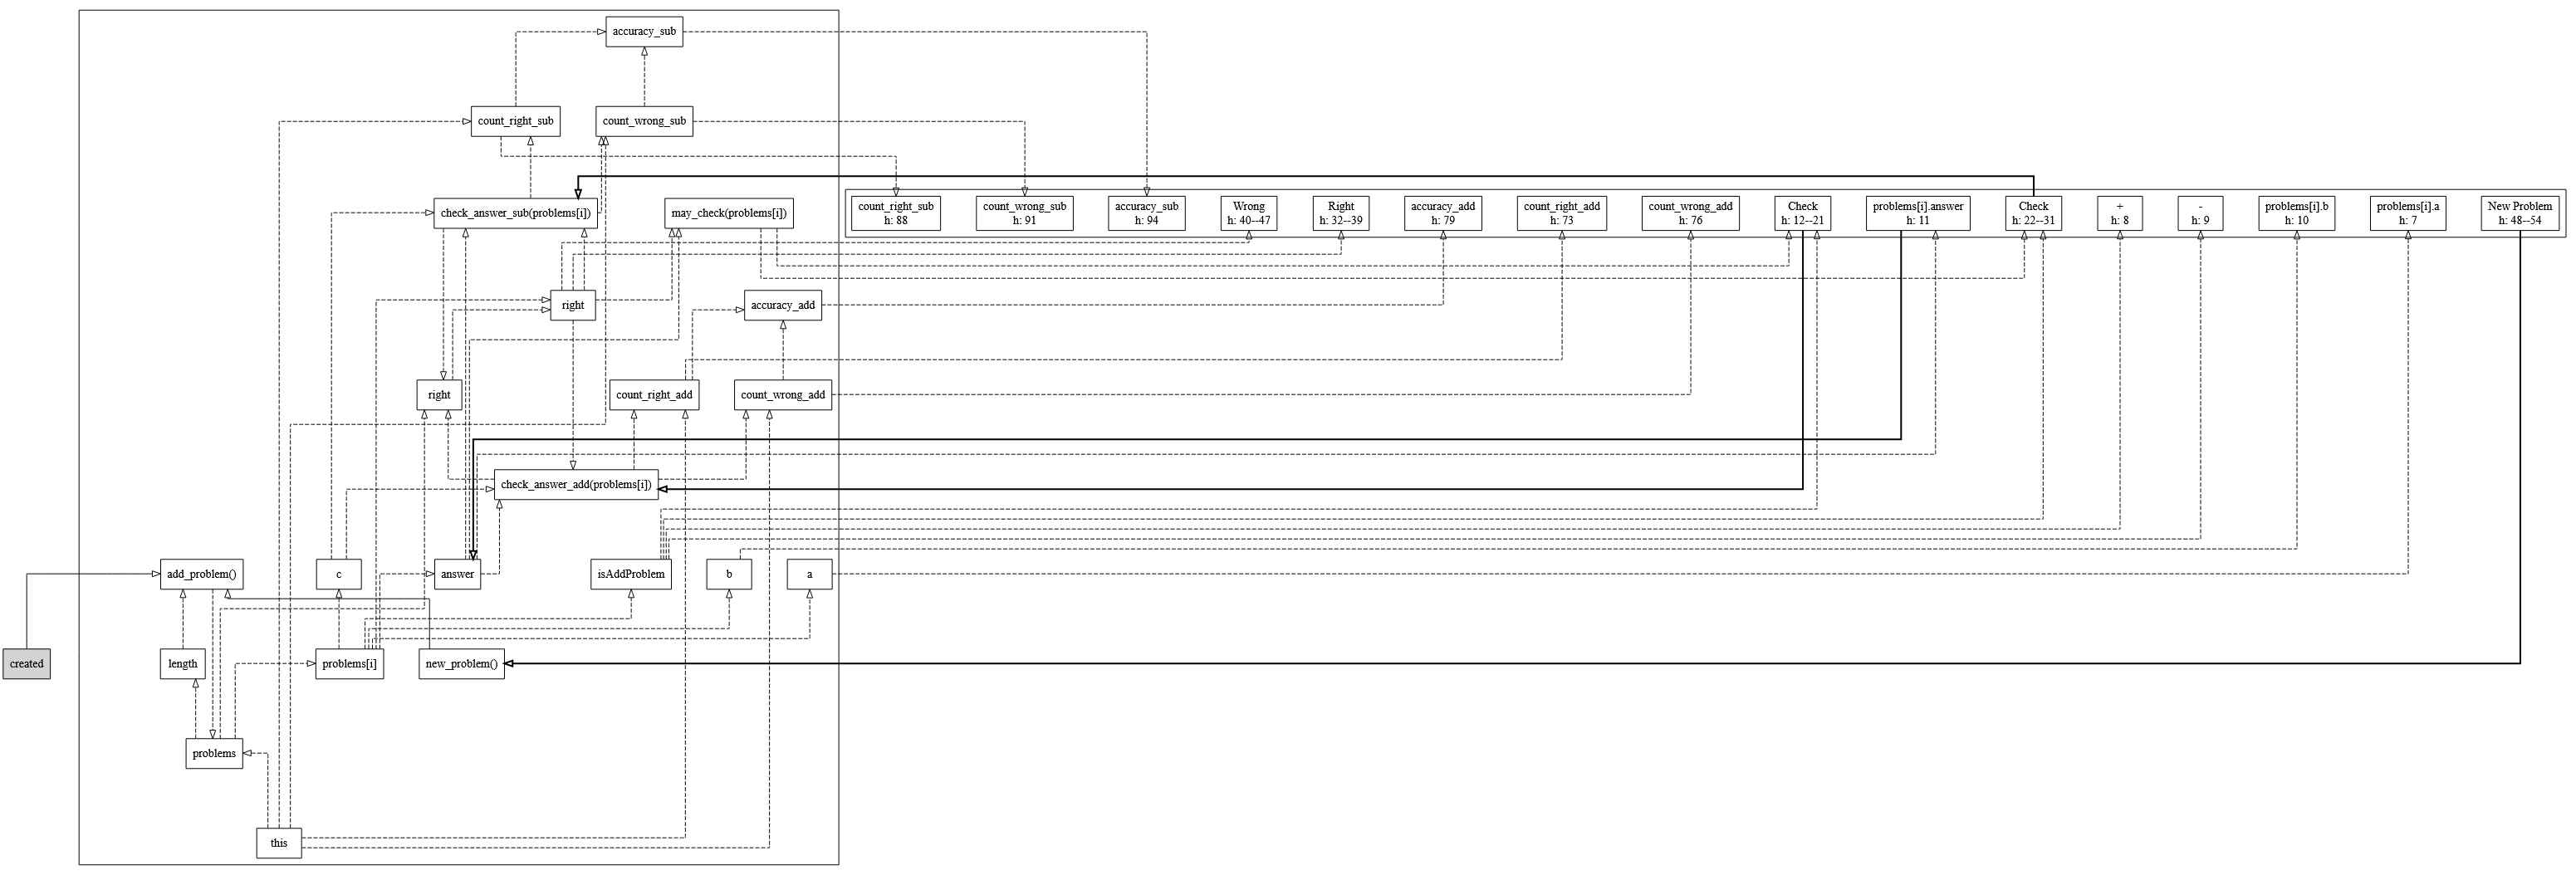
\includegraphics[width=\textwidth]{images/diagram_list_add_sub.png}
     \caption{TODO }
     \label{fig:diagram_test_add_sub}
\end{figure}
